NetData se puede instalar de diferentes maneras, dependiendo del sistema operativo y de las preferencias del usuario. En este caso, se toma la forma de instalación nativa, y con kickstart.sh. A continuación, se describen los pasos para instalar NetData en un sistema Ubuntu Server.

\begin{itemize}
    

\item  Para actualizar la lista de paquetes del sistema se ejecutó el siguiente
comando:

\begin{lstlisting}[style=terminal]
sudo apt update
sudo apt full-upgrade -y
\end{lstlisting}

\item Para instalar NetData, se ejecutó el siguiente comando:

\begin{lstlisting}[style=terminal]
wget -O /tmp/netdata-kickstart.sh https://get.netdata.cloud/kickstart.sh && sh /tmp/netdata-kickstart.sh
\end{lstlisting}

\item Una vez terminada la instalación, se puede acceder a la interfaz web de NetData desde un navegador web, utilizando la dirección IP del servidor y el puerto 19999. Por ejemplo, si la dirección IP del servidor es 10.166.114.156: http://10.166.114.156:19999

\begin{figure}[H]
    \centering
    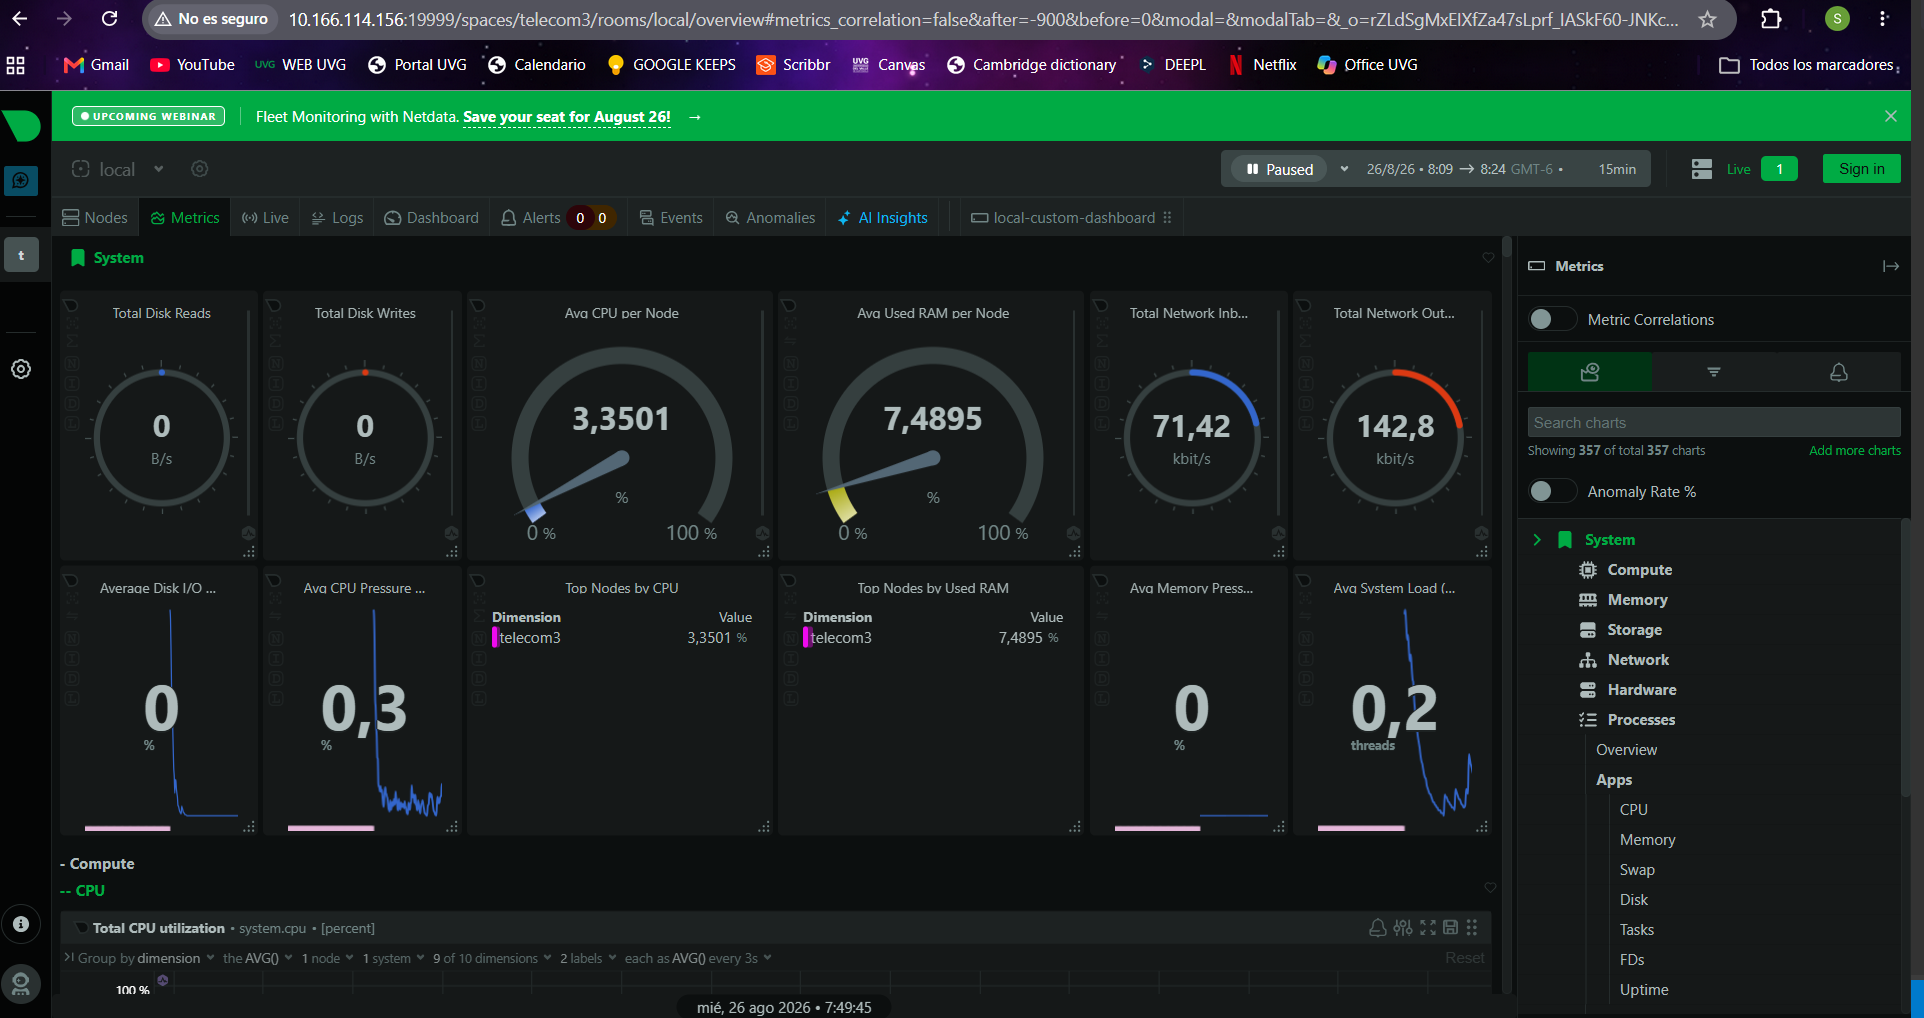
\includegraphics[scale= 0.4]{Pictures/Net.PNG}
    \caption{Tablero de NetData}
    \label{CON1}
\end{figure}

\end{itemize}

